\documentclass{school-22.211-notes}
\date{May 23, 2012}

\begin{document}
\maketitle

%%%%%%%%%%%%%%%%%%%%%%%%% Qualify Exam Start %%%%%%%%%%%%%%%%%%%%%%%%%%%%
\lecture{Facts For Qualify Exam}

\topic{Basics}
\begin{enumerate}
\item Common units, see Table~\ref{units}.
\begin{table}[ht]
  \centering
  \begin{tabular}{|c|c|c|c|c|} \hline
   $\sigma$ & $\Sigma$ & $\phi = nv$ & $R = \phi \Sigma$ & RI  \\ \hline
   $\cm^2$ & $1/\cm$ & $\frac{n}{\cm^2 \s}$ & $\frac{\mathrm{reactions}}{\cm^3 \s}$ & barns \\ \hline
  \end{tabular}
  \caption{Units of Common Terms} \label{units}
\end{table}
\item Fast flux in hydrogen is around $10^{14}$ n/cm$^2$s, and on the order of $10^{12}$n/cm$^2$s for thermal flux. 
\item Average fission neutron energy: 2 MeV; average peak fission energy: 1 MeV; see fission sepctrum. 
\item Core decay heat after 1 day is about 1\% rated. 
\item Constants to know: 1u = 931.5 MeV. 
\item The effect of U238 energy self-shielding is about an effect of 10, that is, going from infinite dilution to U/I = 0.1. 
\end{enumerate}


\clearpage
\topic{Cross Section}
\begin{enumerate}
\item* If the neutron cross section is independent of energy at 0K, at 1200K the cross section would have a 1/v energy shape because of thermal motion. 
  
\item* Resonance absorption cross section dominates resonance scattering cross section most of the time (except U238). 

\item* Fission cross section: U235 fission xs at 0.1 eV and 300K is about 200 barns (200-300 barns); Pu239 fission xs is about 475 barns (380-570 barns). Hence in thermal reactors, Pu absorption should be about twice that of uranium. 

\item Elastic scattering cross section as in Figure~\ref{scatter-xs}
\begin{figure}
  \centering
  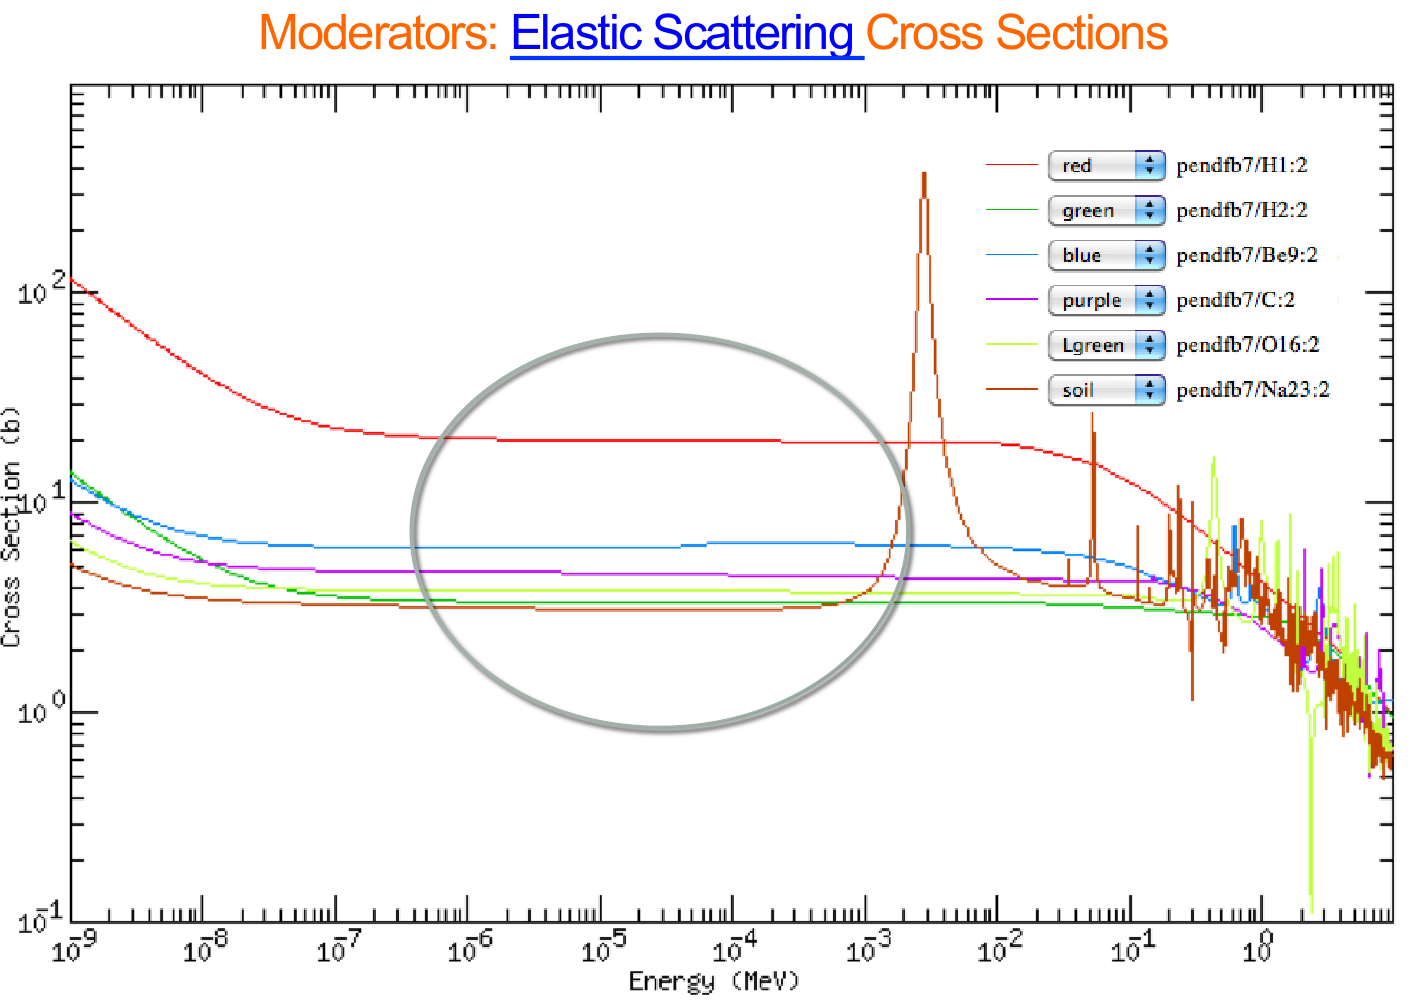
\includegraphics[width=6in]{images/intro/scatter-xs-moderator.png}
  \\
  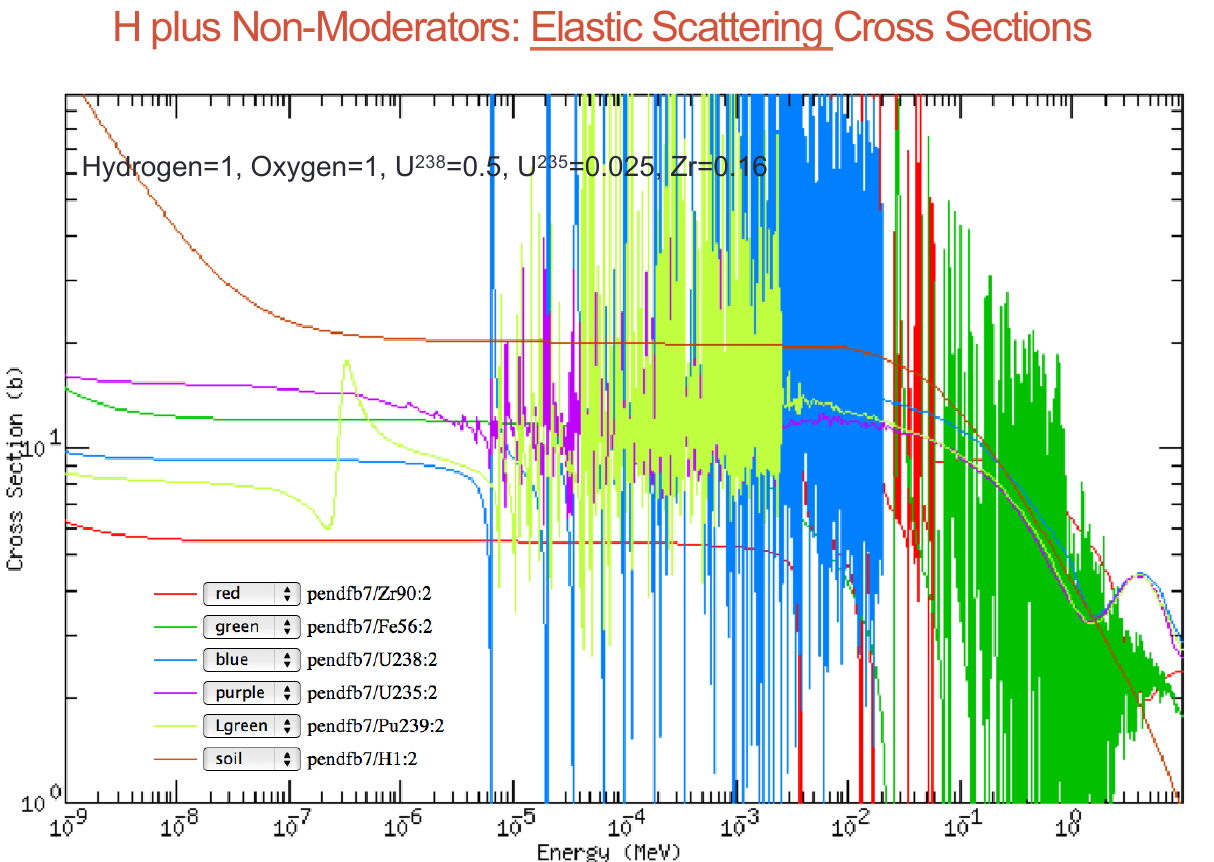
\includegraphics[width=6in]{images/intro/scatter-xs-LWR.png}
  \caption{Elastic Scattering Cross Sections} \label{scatter-xs}
\end{figure}

\item Capture cross section as in Figure~\ref{capture-xs}: 
  \begin{figure}
    \centering
    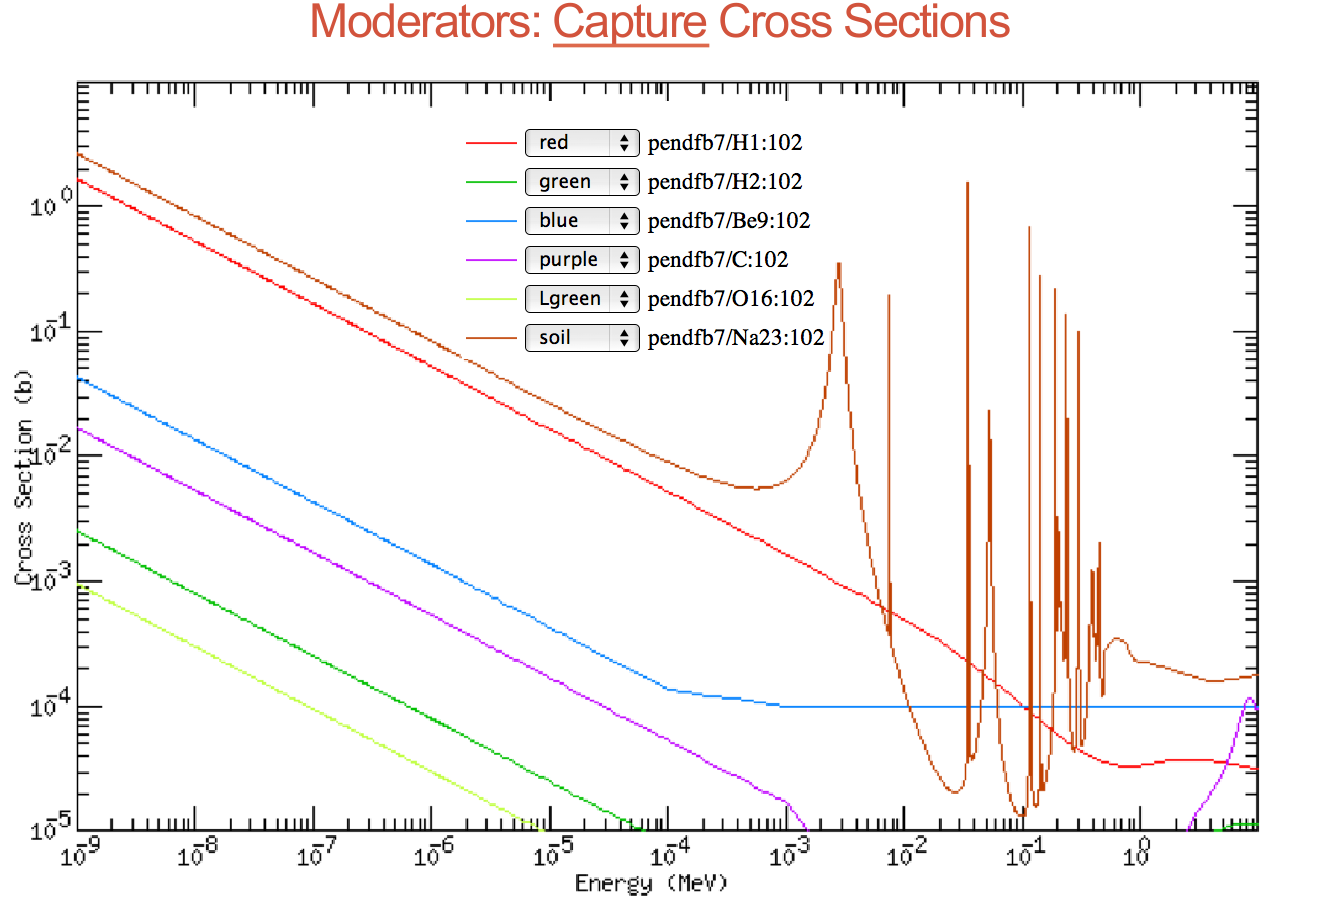
\includegraphics[width=6in]{images/intro/capture-xs.png}
    \\
    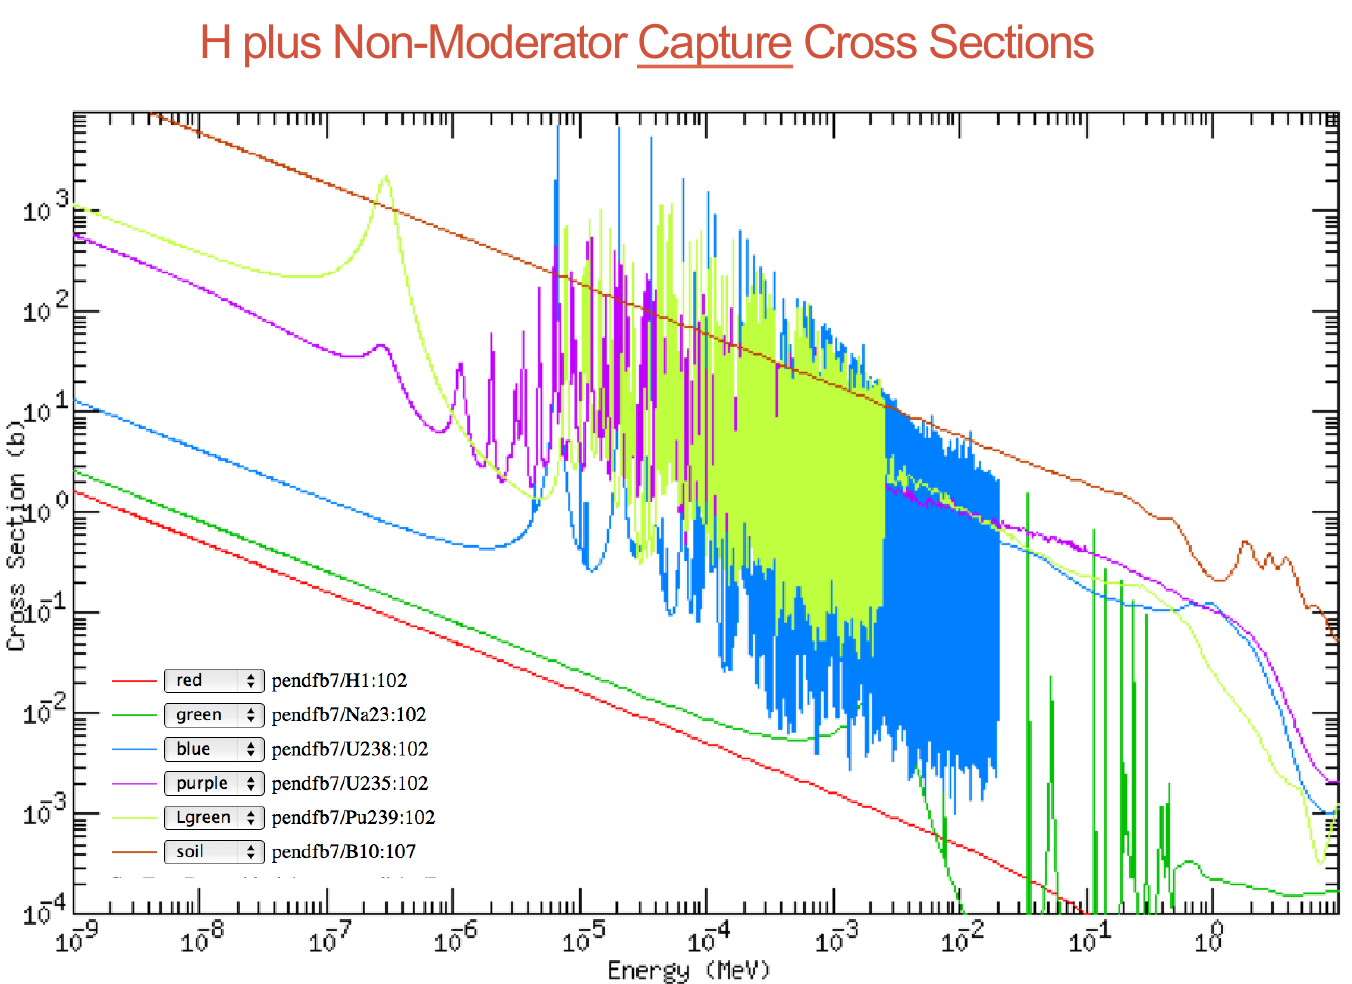
\includegraphics[width=6in]{images/intro/capture-xs-2.png}
    \caption{Capture Cross Section} \label{capture-xs}
  \end{figure}
  \begin{enumerate}
  \item H has no resonance; it has the highest scattering xs in LWR, so we can ignore any other isotopic's neutron scattering.   
  \item Na has a huge resonance in 23 keV, and more resonances at higher energies because it is a heavy isotope.
  \item Near zero energy,
    \eqn{ \sigma(E\to 0) \propto \sqrt{\frac{kT}{AE}}    }
  \item Resonance at 6 to 7 eV: U238. 
  \item U235's thermal elastic xs is larger than 238's, and they both have resonance around the same range.   
  \item A small resonance at .3 eV: Pu239 (its signiture is a super low energy scattering xs). 
  \end{enumerate}

\item Given an unknown material type, all we care is to count the nucleus density of each material and look at it's xs. 
\end{enumerate}


\clearpage
\topic{Kinetics}
\begin{enumerate}
\item PWR 300 pcm/K (Lec10 p. 17, FIXME). 

\item One Group $\kinf$: in one group $k_{\infty}$ only depends on cross sections $k_{\infty} = \frac{\nu \Sigma_f}{\Sigma_a}$ and has no flux dependency. The flux is buried in the calculation of cross section.

\item Two group $\kinf$: we start with neutron balance equation:
  \begin{align}
    \frac{\nu \Sigma_{f1}}{k_{\infty}} \Phi_1 - \Sigma_{a1} \Phi_1 - \Sigma_{s12} \Phi_1 + \frac{\nu \Sigma_{f2}}{k_{\infty}} \Phi_2 + \Sigma_{s21} \Phi_2 &= 0 \\
\Sigma_{s12} \Phi_1 - \Sigma_{s21} \Phi_2 - \Sigma_{a2} \Phi_2 &= 0 
  \end{align}
  Typically what we do is to write it in a matrix form and solve for a coupled system. But even better, we can define the \hi{effective removal rate} $\bar{\Sigma}_{s12}$, and re-write the two-group balance equation: 
  \begin{align}
    \frac{\nu \Sigma_{f1}}{k_{\infty}} \Phi_1 - \Sigma_{a1} \Phi_1 - \bar{\Sigma}_{s12} \Phi_1 + \frac{\nu \Sigma_{f2}}{k_{\infty}} \Phi_2 &= 0 \\
    \bar{\Sigma}_{s12} \Phi_1- \Sigma_{a2} \Phi_2 &= 0 
  \end{align}
  Then we can solve for $\frac{\Phi_1}{\Phi_2}$ from the second equation in terms of cross section, plug in the first equation, and get $k_{\infty}$ from there. Notice that we only know the relative magnitude of $\Phi$ and $\Phi_2$. 

\item Know Two-group diffusion model: group 1 is the fast group larger than 0.625 eV, and group 2 is the thermal group. 
\begin{enumerate}
\item $D_1 = 1.5, D_2 = 0.5$.
\item Total fission source: $\chi_1 = 1.0, \chi_2 = 0.0$ implies that the fission source in thermal group is zero,
  \eqn{ S_f(\vecr) = \chi_g \Sum_g \nu \Sigma_{fg} (\vecr) \phi_g(\vecr) }
\item Scattering source: define effective down-scatter, so up-scattering is zero $\Sigma_{s21} (\vecr) = 0$. 
\item Final Two-Group Diffusion Equations: 
  \eqn{\boxed{ -\divergence D_1 \gradient \phi_1 + [\Sigma_{a1} + \Sigma_{s12} ] \phi_1 = \nu \Sigma_{f1} \phi_1 + \nu \Sigma_{f2} \phi_2 + S_1} }
  \eqn{\boxed{ -\divergence D_2 \gradient \phi_2 + \Sigma_{a2} \phi_2 = \Sigma_{s12} \phi_1 + S_2} }
\end{enumerate}

\item Know the one-group fundamental mode eigenvalues and eigenvectors as in Table~\ref{eigen-values}. 
\begin{table}[ht]
  \centering
  \begin{tabular}{|l|l|l|} \hline
     Slab $\in  \left[- \frac{L}{2}, \frac{L}{2} \right]$ & $\phi(x) = A \cos \left( \frac{\pi x}{L} \right)$ & $B^2 = \left( \frac{\pi}{L} \right)^2$ \\ \hline
     Sphere $\in [0, R]$ & $\phi(r)= A\frac{\sin \left( \frac{\pi r}{R} \right)}{r} $ & $B^2 = \left( \frac{\pi}{R} \right)^2$ \\ \hline
     Infinite cylinder $\in [0, R]$ & $\phi(r) = A J_0 \left( \frac{2.405 r}{R} \right)$ & $B^2 = \left( \frac{2.405}{R} \right)^2$ \\ \hline
     Finite cylinder $r \in [0, R], z \in \left[ -\frac{H}{2}, \frac{H}{2} \right]$ & $\phi(r,z) = A J_0\left( \frac{2.405 r}{R} \right) \cos \left( \frac{\pi z}{H} \right)$ & $B^2 = \left( \frac{2.405}{R} \right)^2 + \left( \frac{\pi}{H} \right)^2$ \\ \hline
     Parallelepiped $\in \left[ -\frac{L_i}{2}, \frac{L_i}{2} \right]$ & $\phi(x) = A \cos \left( \frac{\pi x}{L_x} \right) \cos \left( \frac{\pi y}{L_y} \right) \cos \left( \frac{\pi x}{L_z} \right)$ & $B^2 = \left( \frac{\pi}{L_x} \right)^2 + \left( \frac{\pi}{L_y} \right)^2 + \left( \frac{\pi}{L_z} \right)^2$ \\ \hline
  \end{tabular}
\end{table}

\end{enumerate}



\clearpage
\topic{2011 Qualify Exam Problems}
\begin{enumerate}
\item Steady-state problems. 
\begin{enumerate}
\begin{figure}[ht]
  \centering
  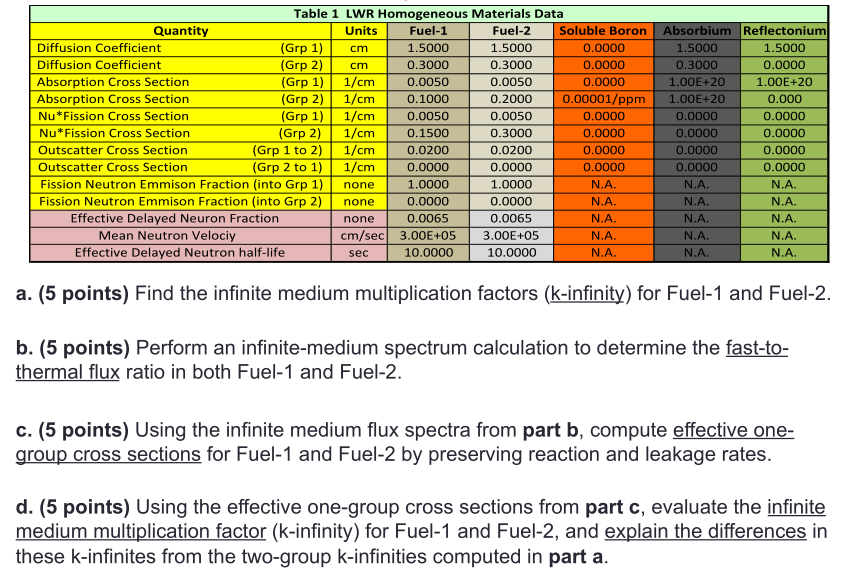
\includegraphics[width=6in]{images/qual/quiz-0.png}
\end{figure}

\item From the two group equations, 
  \begin{align}
    \left\{ \begin{array}{c}
      (\Sigma_{a1} + \Sigma_{s12} ) \phi_1 = \frac{1}{\kinf} ( \nu \Sigma_{f1} \phi_1 + \nu \Sigma_{f2} \phi_2 )   \\
      \Sigma_{a2} \phi_2 = \Sigma_{s12} \phi_1
    \end{array} \right. 
  \end{align}
Then we can solve for the $\kinf$,
\eqn{ \kinf = \frac{\nu \Sigma_{f1} + \nu \Sigma_{f2} \frac{\Sigma_{s12}}{\Sigma_{a2}}}{\Sigma_{a1} + \Sigma_{s12}} }

\item $\frac{\phi_2}{\phi_1} = \frac{\Sigma_{s12}}{\Sigma_{a2}}$. 

\item To preserve reaction rates, $ \Sigma = \frac{\Sum \Sigma \phi}{\Sum \phi}$
  To preserve leakage rates, $D = \frac{\Sum D \phi}{\Sum \phi}$.
 
\item Us the $\nu \bar{\Sigma}_f, \bar{\Sigma}_a$, we can calculate
  \eqn{ \kinf = \frac{\nu \bar{\Sigma}_f}{\bar{\Sigma}_a} }
  The $\kinf$ calculated from effective one-group cross sections is the same as the one calculated from two-group cross sections, because the one-group data is calculated preserving reaction rates. 

\clearpage
\begin{figure}[ht]
  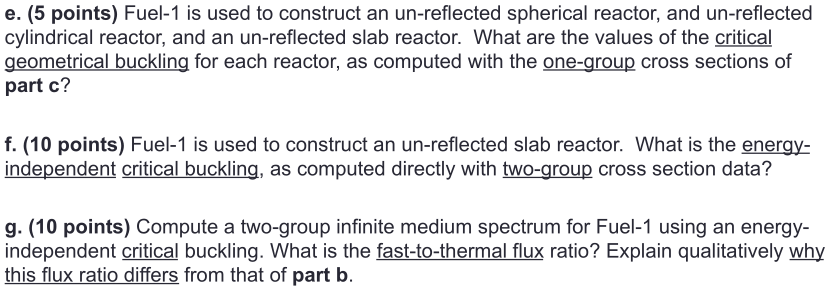
\includegraphics[width=6in]{images/qual/quiz-1.png} 
  \\
  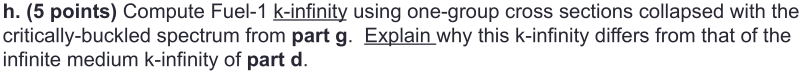
\includegraphics[width=6in]{images/qual/quiz-2.png}
\end{figure}
\item The critical buckling is, 
  \eqn{ B^2 = \frac{\nu \Sigma_f - \Sigma_a}{D} }

\item `unreflected' means that there are leakages now, `energy-independent' means that $B^2$ is the same for group 1 and 2,
  \begin{align}
    \left\{ \begin{array}{c}
      (D_1 B^2 + \Sigma_{a1} + \Sigma_{s12} ) \phi_1 = \frac{1}{\keff} ( \nu \Sigma_{f1} \phi_1 + \nu \Sigma_{f2} \phi_2 )  \\
      (D_2 B^2 +  \Sigma_{a2}) \phi_2 = \Sigma_{s12} \phi_1 
    \end{array} \right. 
  \end{align}
Then we can solve for $B^2$ given $\keff = 1$. 

\item From the above equations taking into account leakage, 
  \eqn{ \frac{\phi_1}{\phi_2} = \frac{D_2 B^2 + \Sigma_{a2}}{\Sigma_{s12}} }
  It is different from part b because the finite unreflected geometry has leakage terms. 

\item The $\kinf$ using one-group cross sections collapsed with the critically-buckled spectrum from part g ($\frac{\phi_1}{\phi_2}$), 
  \eqn{ \kinf = \frac{\nu \Sigma_{f1} \frac{\phi_1}{\phi_2} + \nu \Sigma_{f2} }{\Sigma_{a1} \frac{\phi_1}{\phi_2} + \Sigma_{a2} } }
  This $\kinf$ is smaller then the one in part d because most fission comes from thermal spectrum, and a lot of it leaks out. Notice is is good to double check to make sure that the calculated $\kinf$ result is no larger than $\nu$. 

\clearpage
\begin{figure}[ht]
  \centering
  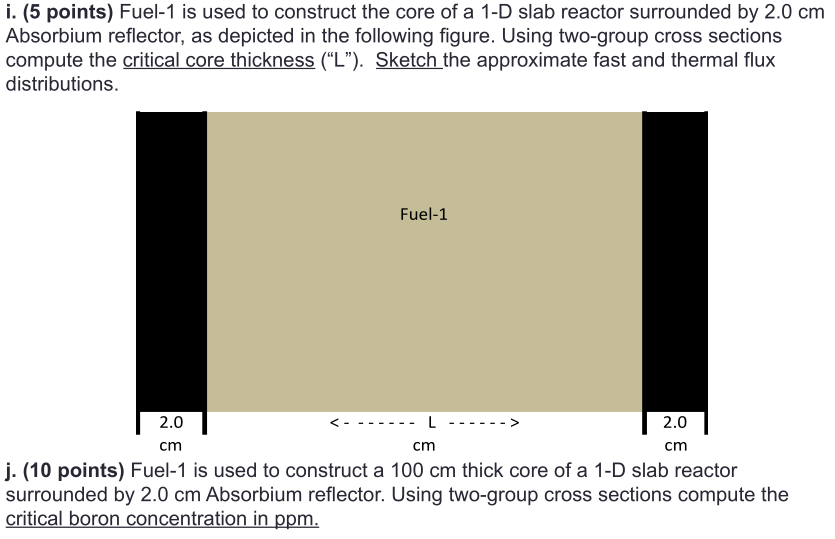
\includegraphics[width=6in]{images/qual/quiz-3.png}
\end{figure}
\item Though this appears to be a multi-region problem. But since the reflector is made of absorbium whose absorption cross section is infinite for both energy groups, the problem is effectively a one-group problem, including the core with length $L$ and the approximated extropolated distance of $2D$ on each side. Hence we solve for, 
  \eqn{ B^2 &= \left( \frac{\pi}{L'} \right)^2, & L &= L' - 4D }

\item There are two approaches. Approach 1: 
  \eqn{ \keff = 1 = \frac{\nu \Sigma_f^F}{DB^2 + N_F \sigma_a^F + N_P \sigma_a^P} }
  Approach 2: we solve for the unknown $\Sigma_a$ that would make $B_m^2 = B_g^2$; then solve for the concentration. 

\clearpage
\begin{figure}[ht]
  \centering
  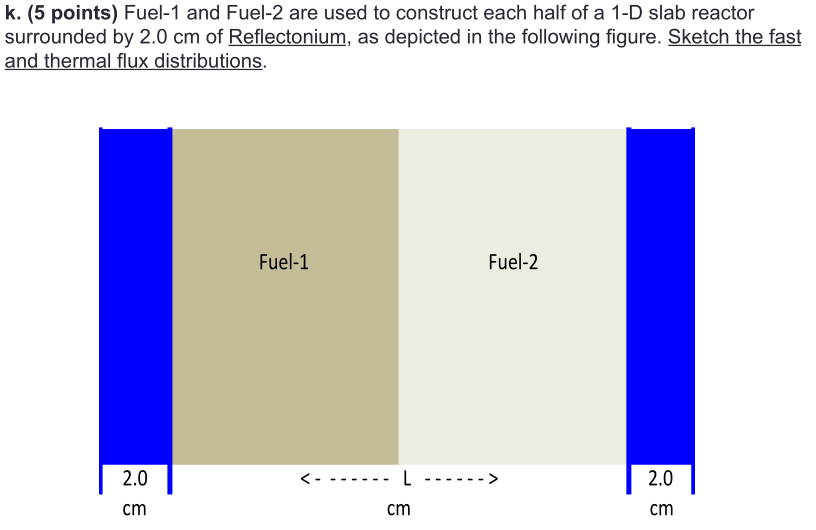
\includegraphics[width=6in]{images/qual/quiz-4.png}  
\end{figure}
\item For the flux shape, 
  \begin{itemize}
    \item Fast energy: flux in the fuel region is cos shape, and suddenly drop to 0 at the interface because the Reflectonium has an infinite large absorption cross section in fast energy. 
    \item Thermal energy: Reflectonium is a perfect reflector for the thermal region, hence the flux's slope should approach zero at the interface. 
  \end{itemize}


\end{enumerate}
\end{enumerate}
%%%%%%%%%%%%%%%%%%%%%%%%% Qualify Exam End %%%%%%%%%%%%%%%%%%%%%%%%%%%%




\end{document}
